There are various manifestations of \gls{soc} observable in the artifacts. One of which is
already mentioned in Figure \ref{fig:modulair_components}, where \gls{soc} is applied to
separate the domain logic from the application, infrastructure and presentation logic.

Another example is the separation of handlers as part of the Clean Architecture Expander.
Each of those handlers executes an isolated part of the expanding process. Consider the
\citetitle{koks_expandentitieshandlerinteractor_2023}
\parencite{koks_expandentitieshandlerinteractor_2023} for example. This Handler is solely
responsible for the generation of Data Entities. 

\begin{figure}[H]
    \centering
    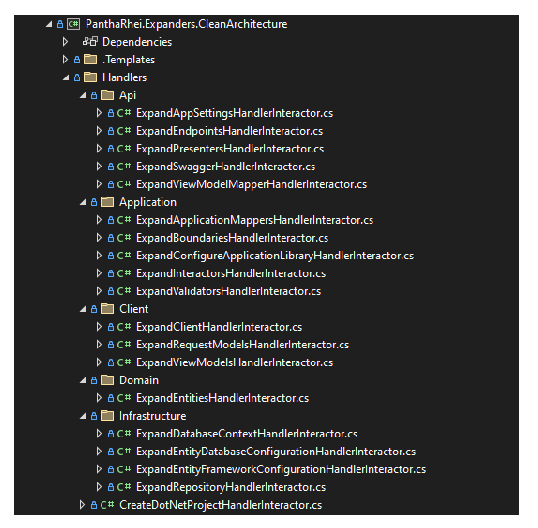
\includegraphics[width=0.8\textwidth]{Figures/expander_handlers.pdf}
    \caption[handlers]{Each of the handlers handles an isolated part of the expanding process.}
    \label{fig:handlers}
\end{figure}